\usetikzlibrary{patterns} % Load patterns library
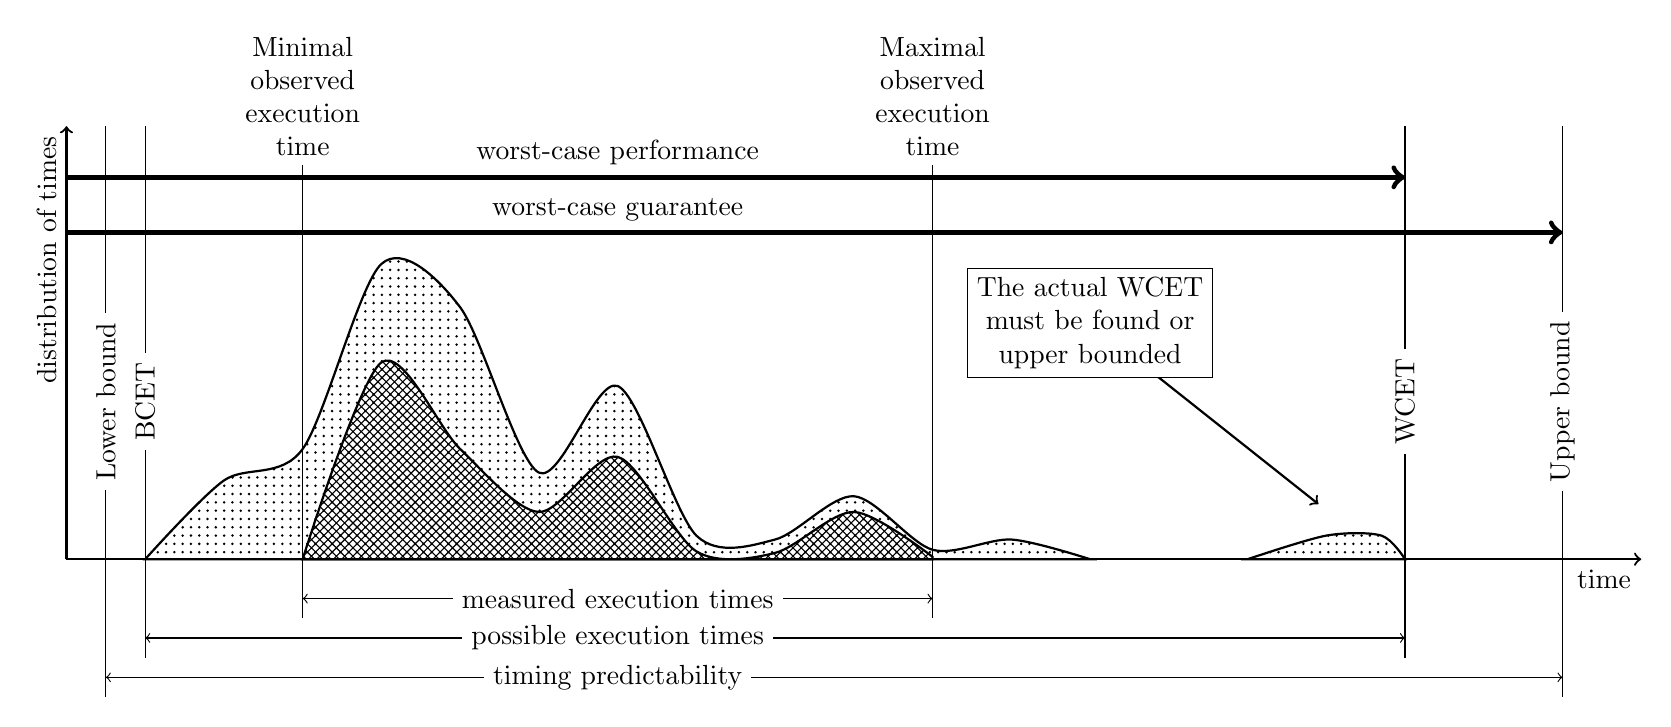
\begin{tikzpicture}
	% Axes
	\draw[->,thick] (0,0) -- (20,0) node[below,anchor=north east]{time};
	\draw[->,thick] (0,0) -- (0,5.5) node[left,rotate=90,anchor=south east]{distribution of times};

	% Execution time distribution (just shape some)
	\draw[thick, fill=black!60, pattern=dots] plot[smooth] coordinates {
	(1,0)
	(2,1)
	(3,1.4)
	(4,3.75)
	(5,3.2)
	(6,1.1)
	(7,2.2)
	(8,0.3)
	(9,0.25)
	(10,0.8)
	(11,0.12)
	(12,0.25)
	(13,0)
	} -- (13,0) -- cycle;
	\draw[thick, fill=black!60, pattern=dots] plot[smooth] coordinates {
	(15,0)
	(16,0.3)
	(16.7,0.3)
	(17,0)
	} -- (17,0) -- cycle;
		% measured times
	\draw[thick, fill=black!30, pattern=crosshatch] plot[smooth] coordinates {
	(3,0)
	(4,2.5)
	(5,1.4)
	(6,0.6)
	(7,1.3)
	(8,0.1)
	(9,0.08)
	(10,0.6)
	(11,0.03)
	} -- (11,0) -- cycle;

	% Vertical markers for BCET, min/max observed times, WCET
	\draw[] (0.5,-1.75) -- (0.5,5.5);
	\node[above,fill=white,align=center,rotate=90,anchor=center] at (0.5,2) {Lower bound};
	\draw[] (1,-1.25) -- (1,5.5);
	\node[above,fill=white,align=center,rotate=90,anchor=center] at (1,2) {BCET};
	\draw[] (3,-0.75) -- (3,5.5);
	\node[above,fill=white,align=center] at (3,5) {Minimal\\observed\\execution\\time};
	\draw[] (11,-0.75) -- (11,5.5);
	\node[above,fill=white,align=center] at (11,5) {Maximal\\observed\\execution\\time};
	\draw[] (17,-1.25) -- (17,5.5);
	\node[above,fill=white,align=center,rotate=90,anchor=center] at (17,2) {WCET};
	\draw[] (19,-1.75) -- (19,5.5);
	\node[above,fill=white,align=center,rotate=90,anchor=center] at (19,2) {Upper bound};

	% Horizontal worst-case performance and guarantee
	\draw[line width=0.7mm,->] (0,4.85) -- (14,4.85) node[midway,above]{worst-case performance} -- (17,4.85);
	\draw[line width=0.7mm,->] (0,4.15) -- (14,4.15) node[midway,above]{worst-case guarantee} -- (19,4.15);

	% Execution time arrows
	\draw[<->] (3,-0.5) -- (11,-0.5) node[midway,fill=white]{measured execution times};
	\draw[<->] (1,-1) -- (3,-1) -- (11,-1) node[midway,fill=white]{possible execution times} -- (17,-1);
	\draw[<->] (0.5,-1.5) -- (3,-1.5) -- (11,-1.5) node[midway,fill=white]{timing predictability} -- (19,-1.5);

	% Annotations
	\draw[->, thick] (13,3) -- (15.9,0.7);  
		\node[draw, fill=white, align=center] at (13,3) {The actual WCET\\ must be found or\\ upper bounded};
	
\end{tikzpicture}